%!TEX root = main.tex

\newpage
\section{Задание}

Синтезировать 4-разрядный ОА, реализующий две операции --- арифметическую и логическую, в соответствии с заданным вариантом (Таблица \ref{table:task}). Работу ОА промоделировать, используя САПР <<Альтера>> Max+plus II.

\begin{table}[H]
	\centering
	\caption{Операции, реализуемые ОА}
	\label{table:task}
	\begin{tabular}{| l | l | l | p{2.2cm} | p{2.2cm} | c | c | c | c | c |} \hline
		\multirow{2}{2cm}{Вариант} & \multirow{2}{2cm}{Операция} & \multirow{2}{2cm}{Код} & \multirow{2}{2.2cm}{Элементы памяти ОА1} & \multirow{2}{2.2cm}{Элементы памяти ОА2} & \multicolumn{5}{c|}{Признаки} \\ \cline{6-10}
		& & & & & S & Z & C' & P & C \\ \hline 
		\multirow{2}{2cm}{2в, 1} & $A \leftarrow A - 1$ & 8421+3 & JK & \multirow{2}{2.2cm}{DC} & + & + & + & + & - \\ \cline{2-4} \cline{6-10}

		& $A \leftarrow A \& B$ & двоичный & JK & & + & + & 0 & + & 0 \\ \hline 
	\end{tabular}
\end{table}


\newpage
\section{Структура ОА}

На этапе структурного синтеза ОА представляют в виде двух частей --- памяти и комбинационной схемы КС (Рисунок \ref{figure:oooa}). КС служит для преобразования входных сигналов Х и информации о состоянии устройства (А) в выходные сигналы Y и сигналы возбуждения элементов памяти U.

\begin{figure}[H]
	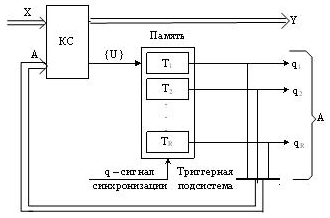
\includegraphics[scale=0.6]{images/2.png}
	\caption{Обобщенная структура ОА}
	\label{figure:oooa}
\end{figure}

Поведение структуры (Рисунок \ref{figure:oooa}) описывается четырьмя группами различных сигналов:

$X$ --- входное слово,

$Y = (X,A)$ --- выходное слово,

$U = \psi(X,A)$ --- слово (функция), обеспечивающее порядок смены состояний автомата

$A$ --- слово, характеризующее состояние автомата.

Внутреннее состояние автомата $А$ определяется состоянием триггеров $a_r \in \{0, 1\}$  и описывается словом состояния $A = (a_1, a_2, a_3, ..., a_i, ... a_r), r = \oline{1,R}$. Множество слов $A$ определяет объем памяти ОА.

Синтезируемый ОА является 4-х разрядным и формирует слово состояния $A = a_3a_2a_1a_0$ .


\newpage
\section{Синтез ОА}

Задача синтеза ОА сводится к:
-   выбору типа элементов памяти (триггеров), который задан заранее (в данной курсовой работе – ТС - триггеры);
- разработке КС, для чего необходимо сформировать систему переключательных функций, описывающую ее поведение:
 ;	                          				                       (1)
-  реализации системы ПФ (1) на заданной элементной базе (в данной курсовой работе используется элементная база САПР MAX+plus II 10.0).
В случае, если автомат оказывается сложным, задачу синтеза ОА упрощают, декомпозируя (разделяя) его на более простые автоматы ОА1 и ОА2 (рис. 3) с одинаковой структурой (рис. 4).

<<<<<<<Рисунок 3 - Декомпозиция ОА>>>>>>>>>

<<<<<<<Рисунок 4 - Структурное представление ОА1 и ОА2>>>>>>>>>

Арифметико-логический автомат ОА1 формирует слово А результата операции и сигналы fS, fC, fZ, fP, fC’ – логические функции признаков (ЛФП), относящиеся к выходным сигналам Y=λ(X,A), на основе которых ОА2 формирует уже сами признаки – слово F=(S, Z, P, C, C’) в соответствии с логикой признаков, которая задается таблично для каждой отдельной операции. Операции, реализуемые ОА (рис. 3), инициализируются управляющими сигналами{yi}. Поскольку сигналы y0, y1 несовместимы во времени, в текущий момент t только один из управляющих сигналов может быть равен 1 ( другой сигнал равен нулю). 


\subsection{Синтез ОА${}_1$}


ОА1 можно рассматривать как многооперационный автомат, способный реализовать не одну, а несколько операций. Синтез автомата ОА1 разделяется на синтез автоматов ОА1(0) и ОА1(1)  с памятью на ТС-триггерах, реализующих соответственно: 
- операцию сложения с переносом (А←А+С) в коде “8421+3”, инициируемую сигналом y0.
- операцию логического сложения с двоичной константой ( 2), инициируемую сигналом y1.
Абстрактное представление ОА1 изображено на рис. 5.

<<<<<<Рисунок 5 –  Абстрактное представление ОА1>>>>>>

Автомат ОА1(0) реализует операцию над одним словом А с установкой результата, поэтому ОА не декомпозируется, и синтезируется как единый 4-х разрядный ОЭ.
Автомат ОА1(1) реализует операцию над двумя 4-х разрядными словами А и В с установкой результата. Сигналы возбуждения и выходов являются функциями восьми аргументов. При рассмотрении такого автомата как единого ОЭ синтез значительно усложнится (КТ будет содержать 256=28 наборов), поэтому ОА1(1)  декомпозируется, и синтезируется как композиция одноразрядных ОЭ.


\subsubsection{Синтез ОА${}_{10}$}



%!TEX root = main.tex
\kvnoindex
\begin{figure}[H]
	\begin{subfigure}[b]{0.3\textwidth}
	\karnaughmap{4}%
	{$J^{(0)}_3:$}%
	{{$a_1$}{$a_3$}{$a_0$}{$a_2$}}%
	{x0x0xxxxx010xxxx}%
	{%
		\textcolor{Blue}{%
			\put(4, 2){\oval(1.9, 3.9)[l]}
			\put(0, 2){\oval(1.9, 3.9)[r]}
		}%
	}
	\caption{}
	\label{figure:oa10_min_J3}
	\end{subfigure}
	\qquad
	\begin{subfigure}[b]{0.3\textwidth}
	\karnaughmap{4}%
	{$K^{(0)}_3:$}%
	{{$a_1$}{$a_3$}{$a_0$}{$a_2$}}%
	{xxxx100xxxxx0x0x}%
	{%
		\textcolor{Blue}{%
			\put(4, 3.5){\oval(1.9, 0.9)[l]}
			\put(0, 3.5){\oval(1.9, 0.9)[r]}
		}%
	}
	\caption{}
	\label{figure:oa10_min_K3}
	\end{subfigure}

	\begin{subfigure}[b]{0.3\textwidth}
	\karnaughmap{4}%
	{$J^{(0)}_2:$}%
	{{$a_1$}{$a_3$}{$a_0$}{$a_2$}}%
	{xxxx1x0xxx1x0x0x}%
	{%
		\textcolor{Blue}{%
			\put(2, 3.5){\oval(3.9, 0.9)[l]}
			\put(2, 3.5){\oval(3.9, 0.9)[r]}
		}%
		\textcolor{Red}{%
			\put(1, 2){\oval(1.9, 3.9)[t]}
			\put(1, 2){\oval(1.9, 3.9)[b]}
		}%
	}
	\caption{}
	\label{figure:oa10_min_J2}
	\end{subfigure}
	\qquad
	\begin{subfigure}[b]{0.3\textwidth}
	\karnaughmap{4}%
	{$K^{(0)}_2:$}%
	{{$a_1$}{$a_3$}{$a_0$}{$a_2$}}%
	{x1x0x1xxx0x0xxxx}%
	{%
		\textcolor{Blue}{%
			\put(2, 3.5){\oval(3.9, 0.9)[l]}
			\put(2, 3.5){\oval(3.9, 0.9)[r]}
		}%
	}
	\caption{}
	\label{figure:oa10_min_K2}
	\end{subfigure}	

	\begin{subfigure}[b]{0.3\textwidth}
	\karnaughmap{4}%
	{$J^{(0)}_1:$}%
	{{$a_1$}{$a_3$}{$a_0$}{$a_2$}}%
	{x1x0110xxxxxxxxx}%
	{%
		\textcolor{Blue}{%
			\put(2, 0){\oval(3.9, 1.9)[t]}
			\put(2, 4){\oval(3.9, 1.9)[b]}
		}%
	}
	\caption{}
	\label{figure:oa10_min_J1}
	\end{subfigure}
	\qquad
	\begin{subfigure}[b]{0.3\textwidth}
	\karnaughmap{4}%
	{$K^{(0)}_1:$}%
	{{$a_1$}{$a_3$}{$a_0$}{$a_2$}}%
	{xxxxxxxxx1101x0x}%
	{%
		\textcolor{Blue}{%
			\put(2, 0){\oval(3.9, 1.9)[t]}
			\put(2, 4){\oval(3.9, 1.9)[b]}
		}%
		\textcolor{Red}{%
			\put(0.5, 2){\oval(0.9, 3.9)[t]}
			\put(0.5, 2){\oval(0.9, 3.9)[b]}
		}%
	}
	\caption{}
	\label{figure:oa10_min_K1}
	\end{subfigure}

	\begin{subfigure}[b]{0.3\textwidth}
	\karnaughmap{4}%
	{$J^{(0)}_0:$}%
	{{$a_1$}{$a_3$}{$a_0$}{$a_2$}}%
	{x1xx11xxx1xx1xxx}%
	{%
		\textcolor{Blue}{%
			\put(2, 2){\oval(3.9, 3.9)[l]}
			\put(2, 2){\oval(3.9, 3.9)[r]}
		}%
	}
	\caption{}
	\label{figure:oa10_min_J0}
	\end{subfigure}
	\qquad
	\begin{subfigure}[b]{0.3\textwidth}
	\karnaughmap{4}%
	{$K^{(0)}_0:$}%
	{{$a_1$}{$a_3$}{$a_0$}{$a_2$}}%
	{xxx1xx1xxx11xx1x}%
	{%
	{%
		\textcolor{Blue}{%
			\put(2, 2){\oval(3.9, 3.9)[l]}
			\put(2, 2){\oval(3.9, 3.9)[r]}
		}%
	}	
	}
	\caption{}
	\label{figure:oa10_min_K0}
	\end{subfigure}	
	
	\caption{Карты Карно для ФВ ОА$^{(0)}_{1}$}
	\label{figure:oa10_min_trig}
\end{figure}

\begin{figure}[H]
	\begin{subfigure}[b]{0.3\textwidth}
	\karnaughmap{4}%
	{$f^{(0)}_s:$}%
	{{$a_1$}{$a_3$}{$a_0$}{$a_2$}}%
	{x0x0011xx0101x1x}%
	{%
		{%
		\textcolor{Blue}{%
			\put(4, 1){\oval(1.9, 1.9)[l]}
			\put(0, 1){\oval(1.9, 1.9)[r]}
		}%
		\textcolor{Red}{%
			\put(3, 2){\oval(1.9, 1.9)[l]}
			\put(3, 2){\oval(1.9, 1.9)[r]}
		}%
		\textcolor{Green}{%
			\put(2.5, 2){\oval(0.9, 3.9)[t]}
			\put(2.5, 2){\oval(0.9, 3.9)[b]}
		}%
	}
	}
	\caption{}
	\label{figure:oa10_min_fs}
	\end{subfigure}
	\qquad
	\begin{subfigure}[b]{0.3\textwidth}
	\karnaughmap{4}%
	{$f^{(0)}_z:$}%
	{{$a_1$}{$a_3$}{$a_0$}{$a_2$}}%
	{x1x0000xx0000x0x}%
	{%
		{%
		\textcolor{Blue}{%
			\put(1, 3.5){\oval(1.9, 0.9)[l]}
			\put(1, 3.5){\oval(1.9, 0.9)[r]}
		}%
		}
	}
	\caption{}
	\label{figure:oa10_min_fz}
	\end{subfigure}

	\begin{subfigure}[b]{0.3\textwidth}
	\karnaughmap{4}%
	{$f_c:$}%
	{{$a_1$}{$a_3$}{$a_0$}{$a_2$}}%
	{x0x0000xx0100x0x}%
	{%
	\textcolor{Blue}{%
			\put(0.5, 2){\oval(0.9, 3.9)[t]}
			\put(0.5, 2){\oval(0.9, 3.9)[b]}
		}%
	}
	\caption{}
	\label{figure:oa10_min_fc}
	\end{subfigure}
	\qquad
	\begin{subfigure}[b]{0.3\textwidth}
	\karnaughmap{4}%
	{$f^{(0)}_p:$}%
	{{$a_1$}{$a_3$}{$a_0$}{$a_2$}}%
	{x1x0000xx1111x1x}%
	{%
		{%
		\textcolor{Blue}{%
			\put(2, 1){\oval(3.9, 1.9)[l]}
			\put(2, 1){\oval(3.9, 1.9)[r]}
		}%
		\textcolor{Red}{%
			\put(1, 0){\oval(1.9, 1.9)[t]}
			\put(1, 4){\oval(1.9, 1.9)[b]}
		}%
	}
	}
	\caption{}
	\label{figure:oa10_min_fp}
	\end{subfigure}	
	
	\begin{subfigure}[b]{0.3\textwidth}
	\karnaughmap{4}%
	{$f^{(0)}_{c'}:$}%
	{{$a_1$}{$a_3$}{$a_0$}{$a_2$}}%
	{x100110xx0x00x0x}%
	{%
		{%
		\textcolor{Blue}{%
			\put(2, 3.5){\oval(3.9, 0.9)[l]}
			\put(2, 3.5){\oval(3.9, 0.9)[r]}
		}%
	}
	}
	\caption{}
	\label{figure:oa10_min_fc1}
	\end{subfigure}

	\caption{Карты Карно для ЛФП ОА$^{(0)}_{1}$}
	\label{figure:oa10_min_flags}
\end{figure}


\subsubsection{Синтез ОА${}_{11}$}

%!TEX root = main.tex

\begin{figure}[H]
\begin{subfigure}[b]{0.3\textwidth}

	\karnaughmap{2}%
	{$J_i:$}%
	{{$b$}{$a$}}%
	{0x0x}%
	{%
	}
	\caption{}
	\label{oa11_J}
\end{subfigure}
\begin{subfigure}[b]{0.3\textwidth}
	\karnaughmap{2}%
	{$K_i:$}%
	{{$b$}{$a$}}%
	{x1x0}%
	{%
	\textcolor{Blue}{
		\put(1,1.5){\oval(1.9,0.9)[]}}
	}
	\caption{}
	\label{oa11_K}
\end{subfigure}
	\caption{oa11mintrig}
	\label{figure:oa11_min_trig}
\end{figure}


\begin{figure}[H]
	\begin{subfigure}[b]{0.3\textwidth}
	\karnaughmap{4}%
	{$f_s:$}%
	{{$r_1$}{$r_3$}{$r_0$}{$r_2$}}%
	{0000111100001111}%
	{%
		\textcolor{Blue}{%
			\put(3, 2){\oval(1.9, 3.9)[t]}
			\put(3, 2){\oval(1.9, 3.9)[b]}
		}%
	}
	\caption{}
	\label{figure:oa11_min_fs}
	\end{subfigure}
	\qquad
	\begin{subfigure}[b]{0.3\textwidth}
	\karnaughmap{4}%
	{$f_z:$}%
	{{$r_1$}{$r_3$}{$r_0$}{$r_2$}}%
	{1000000000000000}%
	{%
		\textcolor{Blue}{
			\put(0.5,3.5){\oval(0.9,0.9)[]}%
		}%	
	}
	\caption{}
	\label{figure:oa11_min_fz}
	\end{subfigure}

	\begin{subfigure}[b]{0.3\textwidth}
	\karnaughmap{4}%
	{$f_p:$}%
	{{$r_1$}{$r_3$}{$r_0$}{$r_2$}}%
	{1001011001101001}%
	{%
		\textcolor{Blue}{
			\put(0.5,3.5){\oval(0.9,0.9)[]}%
			\put(2.5,3.5){\oval(0.9,0.9)[]}%
			\put(1.5,2.5){\oval(0.9,0.9)[]}%
			\put(3.5,2.5){\oval(0.9,0.9)[]}%
			\put(0.5,1.5){\oval(0.9,0.9)[]}%
			\put(2.5,1.5){\oval(0.9,0.9)[]}%
			\put(1.5,0.5){\oval(0.9,0.9)[]}%
			\put(3.5,0.5){\oval(0.9,0.9)[]}%
		}%	
	}
	\caption{}
	\label{figure:oa11_min_fp}
	\end{subfigure}

	\begin{subfigure}[b]{0.3\textwidth}
	\karnaughmap{4}%
	{$f_c:$}%
	{{$r_1$}{$r_3$}{$r_0$}{$r_2$}}%
	{0000000000000000}%
	{}
	
	\caption{}
	\label{figure:oa11_min_fc}
	\end{subfigure}
	\qquad
	\begin{subfigure}[b]{0.3\textwidth}
	\karnaughmap{4}%
	{$f'_c:$}%
	{{$r_1$}{$r_3$}{$r_0$}{$r_2$}}%
	{0000000000000000}%
	{}


	\caption{}
	\label{figure:oa11_min_fc1}
	\end{subfigure}


	\caption{oa11minflags}
	\label{figure:oa11_min_flag}

\end{figure}

\subsubsection{Объединенные ФВ И ЛФП ОА${}_1$}

\subsection{Синтез ОА${}_2$}
